\documentclass[12pt]{article}
\usepackage{graphicx} % For including images
\usepackage[margin=1in]{geometry} % For setting page margins
\usepackage{amsmath} % For extended mathematical formatting
\usepackage{fancyhdr} % For custom headers and footers
\usepackage{float} 
\usepackage{subcaption} % Updated to use subcaption instead of subfigure
\setlength{\headheight}{15pt} % Adjust headheight as recommended
\pagestyle{fancy}
\fancyhf{}
\rhead{EE569 Digital Image Processing}
\lhead{HOMEWORK \#3}
\rfoot{Page \thepage}
\usepackage{enumitem}
\setlist[itemize]{font=\bfseries} 
\begin{document}
	
	\begin{center}
		\Large
		\textbf{Homework \#4}
		
		\vspace{0.2cm}
		\normalsize
		Issued: 02/19/2024 \hfill Due: 03/29/2024
	\end{center}
	
	\section*{Problem 1: Texture Analysis}
		\subsection*{(a) Texture Classification - Feature Extraction}
			Actually it is hard to say which one has the strongest discriminant power: some of them seems can classify correctly in some cases, but also has a lot of false cases. For example, S5*R5. However, it is easy to find that the weakest is L5*L5. The feature remains very high and varies little in all 36 pictures. 
		\subsection*{(b) Advanced Texture Classification --- Classifier Exploration}
		\begin{itemize}[label=$\bullet$]
			\item \textbf{1. Unsupervised Learning}  In the 25-D energy features' kmeans unsupervised learning, test cases are divided into 4 groups: \{1,9\},\{2,3,4,5,6,7, 12\},\{8,11\} and \{10\}. In this cases, group 1 is classified as Brick, group 2 is classified as Grass, group 3 and 4 should be calssified as Blanket or Stones. The final error rate for 25-D energy k-means learning is 50%.\\
			Then we go to the pca 3-D features' unsupervised leraning. The test cases are divided into 4 groups: \{1, 8, 9, 11\},\{2,4,6,7,12\}, \{3,5\} and \{10\}. In this case, Group 1 should be classified as Brick, Group 2 as Grass, Group 3 as Stones and Group 4 as Blanket. The finial error rate for 3-D kmeans unsupervised learning is 41.67\%, which is a bit lower than without pca transferred.\\
			In this case, the application of pca dimension reduction decreases the error rate by one case.  
			
			\item \textbf{2. Supervised Learning} In supervised learninig, when dimension reduction is not applied, the error rate is 25\%. Picture 2,3,4,5,6,7,8,9 and 12 are classified percisely. However, when applied pca to reduce dimensions, the error rate increases to 58.3\% , with only picture 5,6,7,10 and 12 classified correctly. When compaired to unsupervised learning, using 25 dimension in supervised learning is the learning ide with the highest accuracy, while using pca in supervised learning has the lowest. 
		\end{itemize}
	\section*{Problem 2: Texture Segmentation}
		\subsection*{(a) Basic Texture Segmentation}
		\begin{figure}[H]
			\centering 
			\begin{subfigure}{0.4\textwidth}
				\centering
				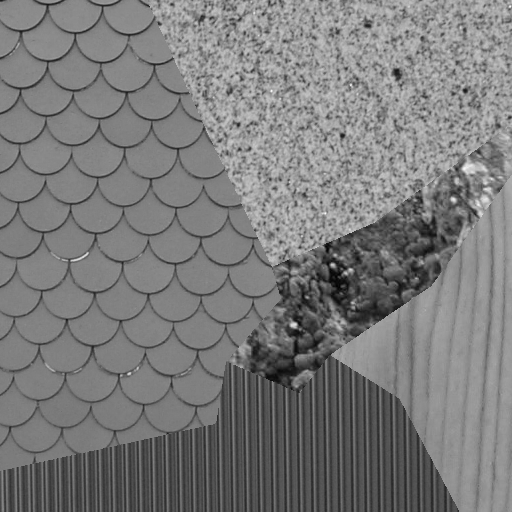
\includegraphics[width=\textwidth]{composite.png}
				\caption{Original Mosiac Image}
				\label{fig:originalmosaic}
			\end{subfigure}
			\hfill
			\begin{subfigure}{0.55\textwidth}
				\centering
				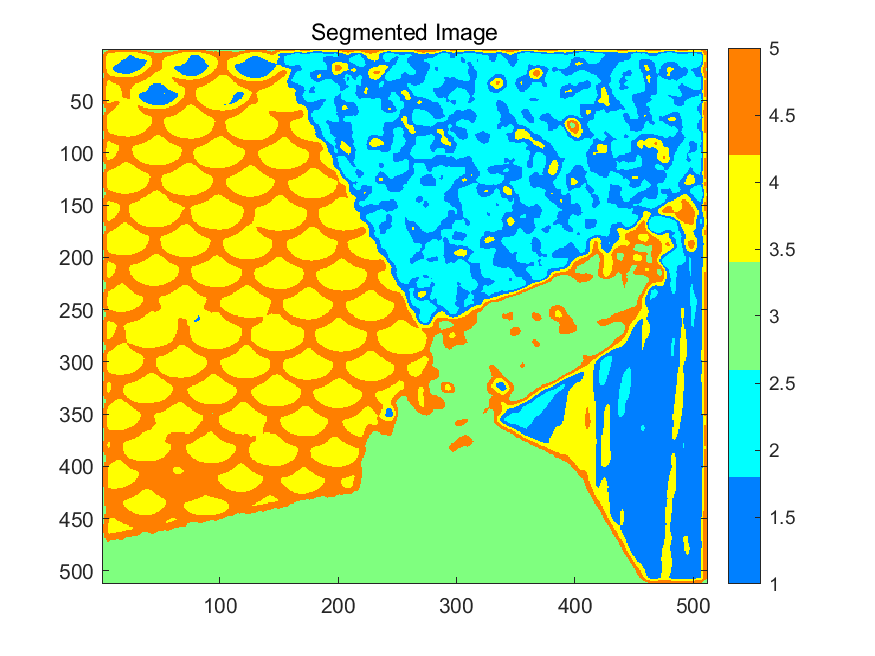
\includegraphics[width=\textwidth]{segmented_image_a.png}
				\caption{Texture Segmentation Image}
				\label{fig:segmentaion}
			\end{subfigure}
			\caption{Texture Segementation}
			\label{p1.1}
		\end{figure}
	\subsection*{(b) Advanced Texture Segmentation}
		In this case, we applied pca dimension-reduction to reduce the interruption of unimportant features. Besides, a post-processing technique that could stop taking small regions into consideration. Beside, edge enhancement is also applied. However, the segmentation still could not regononize the pattern on the left part of the Mosiac Image, where dark lines on light ground forms the texture. It still recognize the lines as a new texture. An idea to solve the problem is to us more improved algorithm, incluing SIFT or CNN learning. 
		\begin{figure}[H]
			\centering
			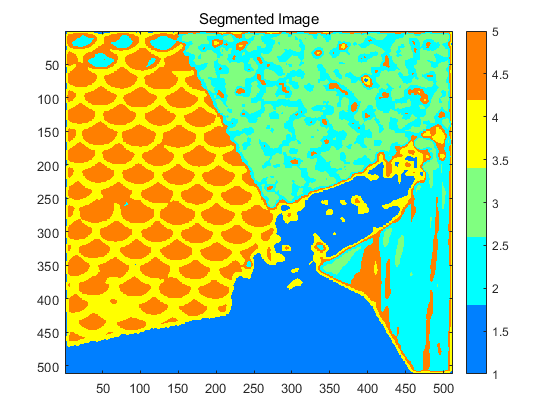
\includegraphics[width=0.5\textwidth]{segmented_image_b.png}
			\caption{Segmentation Image after Improved}
			\label{fig:segementaion2}
		\end{figure}
	\section{Problem 3: SIFT and Image Matching}
		\subsection*{(a) Salient Point Descriptor}
		\begin{itemize}
			\item[1.] From the abstract, we learn that the SIFT could prevent interrupt from image rescaling and rotation, and has robostnesss agains substantial range of affine distortion,change in 3D viewpoint, addition of noise, and change in illumination. Among them, image rescaling, rotation and distortion are geometric modifications.
			
			\item[2.] By taking Difference of Gaussian into consideration, each feature points are compared not only to the pixels next to them on the same scale, but also the points around it before and after rescaling. In this method, SIFT achieves Robustness of rescaling. \\
			For rotation, SIFT adpats a method that could calculate a histogram of orientation. So it could pick a dominant orientation no matter how the image is rotated. 
			
			\item[3.] SIFT enhances its robustness to illumination change by normalizing the feature vectors to unit length, which cancels out the effects of changes in image contrast.  Also, it reduces the influence of large gradient magnitudes caused by non-linear illumination changes through thresholding the values in the unit feature vector and renormalizing it to unit length. These methods emphasizes the distribution of orientations rather than matching the magnitudes for large gradients, making SIFT descriptors more robust to illumination variations.
			
			\item[4.] Laplacian of Gaussian requires more calculation, since smoothed images, L, need to be computed in any case for scalespace feature description, while D can be computed by simple image subtraction, fastening the calculation and remains as a good approximation of the points.
			
			\item[5.] The size is 128.
		
		\end{itemize}
			
		\subsection*{(b) Image Matching}
				\begin{figure}[H]
				\centering 
				\begin{subfigure}{\textwidth}
					\centering
					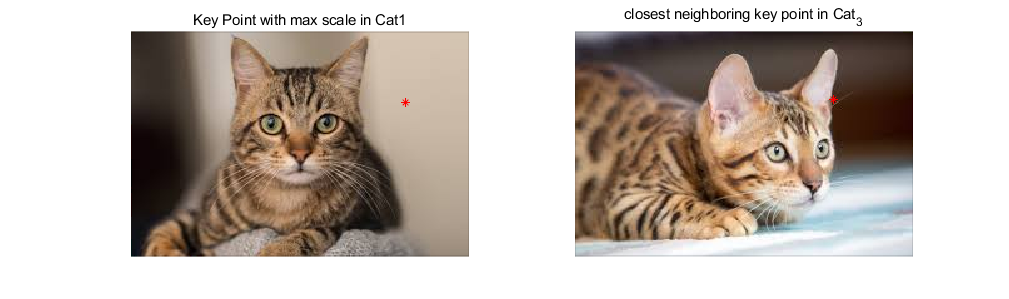
\includegraphics[width=\textwidth]{i11.png}
					\caption{Key point with max scale on Cat 1 and its neighbor in Cat3}
					\label{fig:cat1maxcat3}
				\end{subfigure}
			\\
				\hfill
				\begin{subfigure}{\textwidth}
					\centering
					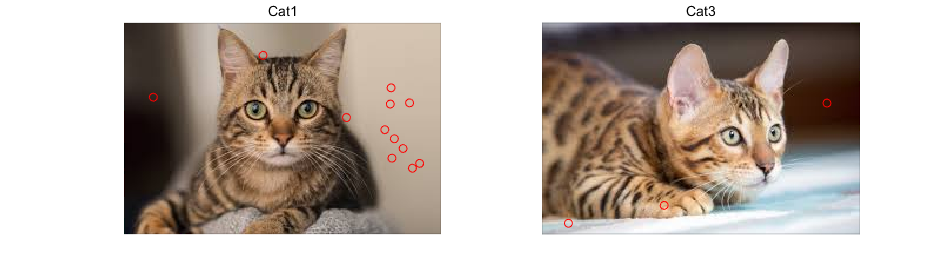
\includegraphics[width=\textwidth]{i12.png}
					\caption{Key points pairs on cat 1 and cat 3}
					\label{fig:cat1cat3}
				\end{subfigure}
			\\
			\hfill
			\begin{subfigure}{\textwidth}
				\centering
				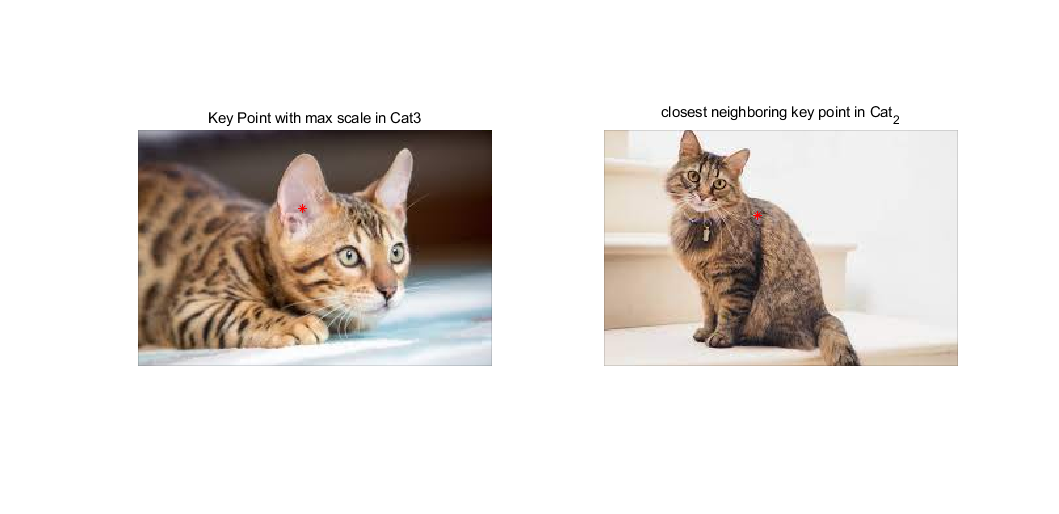
\includegraphics[width=\textwidth]{i21.png}
				\caption{Key point with max scale on Cat 3 and its neighbor in Cat2}
				\label{fig:cat3maxcat2}
			\end{subfigure}
		\\
		\hfill
		\begin{subfigure}{\textwidth}
			\centering
			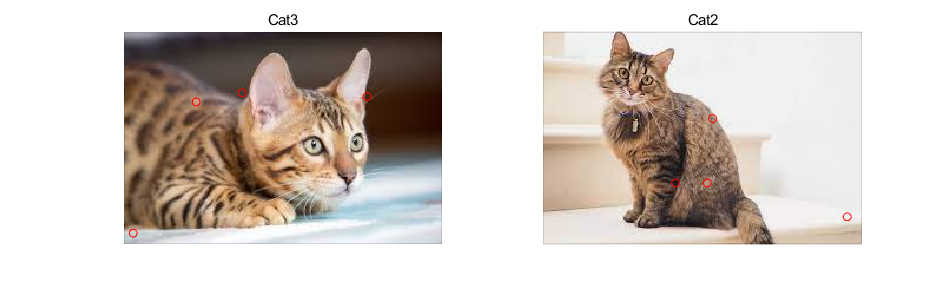
\includegraphics[width=\textwidth]{i22.png}
			\caption{Key points pairs on cat 2 and cat 3}
			\label{fig:cat3cat2}
		\end{subfigure}
	\\\end{figure}
\begin{figure}[H]
		\hfill
		\begin{subfigure}{\textwidth}
			\centering
			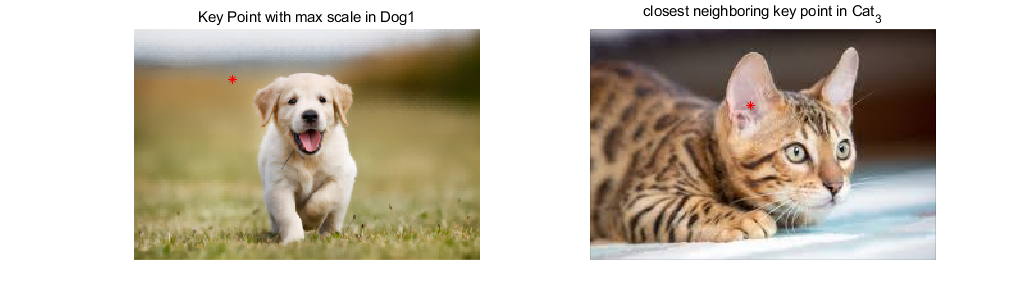
\includegraphics[width=\textwidth]{i31.png}
			\caption{Key point with max scale on Dog1 and its neighbor in Cat3}
			\label{fig:cat3dog1}
		\end{subfigure}
		\\
		\hfill
		\begin{subfigure}{\textwidth}
			\centering
			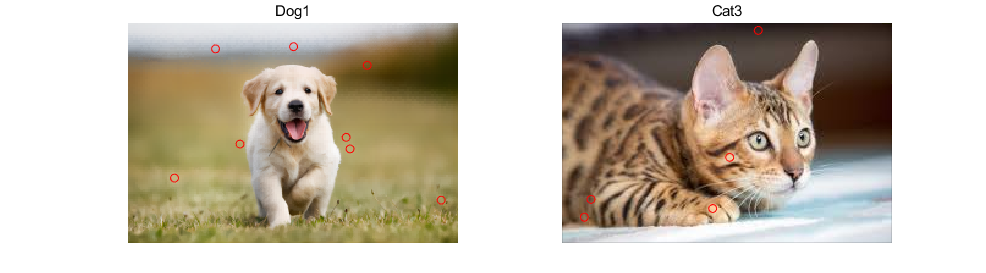
\includegraphics[width=\textwidth]{i32.png}
			\caption{Key points pairs on cat 3 and dog1}
			\label{fig:cat3god3}
		\end{subfigure}
	\\
		\hfill
		\begin{subfigure}{\textwidth}
			\centering
			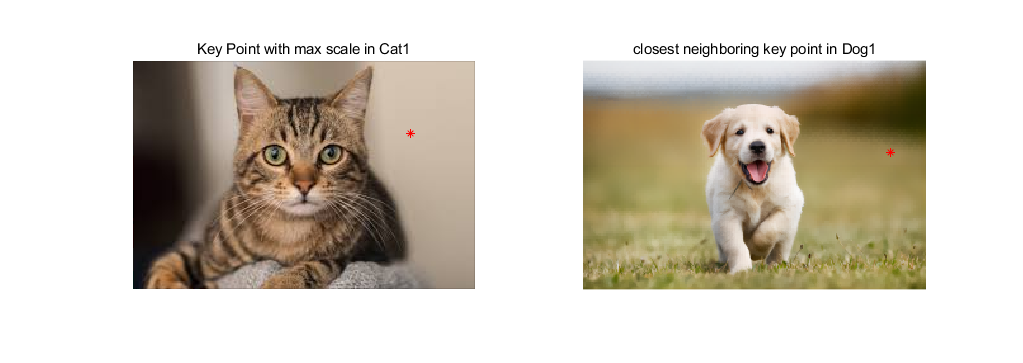
\includegraphics[width=\textwidth]{i41.png}
			\caption{Key point with max scale on Cat 1 and its neighbor in Dog1}
			\label{fig:cat1cmaxdog1}
		\end{subfigure}
		\\
		\hfill
		\begin{subfigure}{\textwidth}
			\centering
			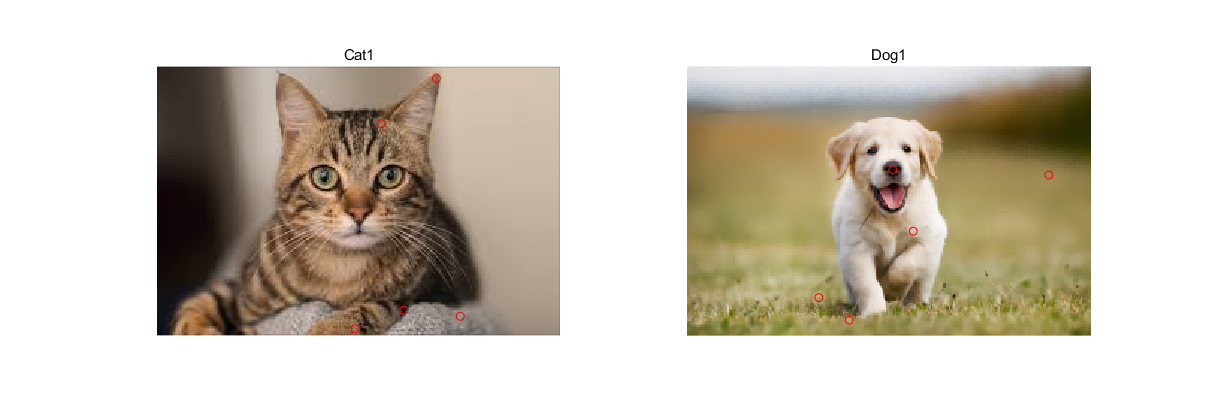
\includegraphics[width=\textwidth]{i42.png}
			\caption{Key points pairs on cat 1 and dog1}
			\label{fig:cat1dog1}
		\end{subfigure}
				\caption{3(b) SIFT key points of fig 4.}
				\label{p1.2}
			\end{figure}
		\subsection*{(c) Bag of Words}
		The outcome:\\
		Similarity of Cat3 codewords to other images:\\
		Similarity to Cat1: 10.6771\\
		Similarity to Cat2: 9\\
		Similarity to Dog1: 175.2199\\
		We find the SIFT could classify the bodies of the picture very well: at least it could tell dog from a ginger-colored cat with black strips. 
		
\end{document}